\chapter{Background}
\label{ch:background}
In this chapter, we define some basic terminology that is used throughout this thesis.

\section{Code clone terminology}\label{sec:terminology}
Many studies present different definitions for code clone concepts. For this study, we mainly use the definitions from Bruntink et al. \cite{bruntink2005use} and Jiang et al. \cite{jiang2007deckard}. A summary of these concepts can be found in Table~\ref{tab:clone-terminology}. The terminology displayed in this table shows how tokens in code map to clones. When detecting clones of a software system, we end up with a clone class collection. Each clone class denotes a set of duplicate fragments. We call these duplicate fragments clone instances. Each clone instance spans several statements/declarations. We refer to these statements and declarations as ``nodes''. Each node consists of a set of tokens.

\begin{table}[H]
\centering
%\resizebox{\textwidth}{!}{%
\begin{tabular}{@{}lllll@{}}
\toprule
\rowcolor[HTML]{FFFFFF}
\textbf{Symbol} & \textbf{Meaning} & \textbf{Definition} & \textbf{Description} \\ \midrule
\rowcolor[HTML]{EFEFEF}
T & Token & - & \begin{tabular}[c]{@{}l@{}}Tokens are the basic lexical\\ building blocks of source code. \\ For this study, this is the smallest\\ relevant entity of a program.\end{tabular} \\
\rowcolor[HTML]{FFFFFF}
N & Node \cite{jiang2007deckard} & Set of tokens. & \begin{tabular}[c]{@{}l@{}}A statement or declaration node\\in the AST of a codebase.\end{tabular}  \\
\rowcolor[HTML]{EFEFEF}
I & \begin{tabular}[c]{@{}l@{}}Clone\\ instance \cite{bruntink2005use}\end{tabular} & \begin{tabular}[c]{@{}l@{}}Set of cloned\\nodes.\end{tabular} & \begin{tabular}[c]{@{}l@{}}A code fragment that appears in\\ multiple locations.\end{tabular} \\
\rowcolor[HTML]{FFFFFF}
C & Clone class \cite{bruntink2005use}& \begin{tabular}[c]{@{}l@{}}Set of clone\\instances.\end{tabular} & \begin{tabular}[c]{@{}l@{}}A set of similar code fragments in\\ different locations. Each of these\\code fragments is called a\\``clone instance''.\end{tabular} \\
\rowcolor[HTML]{EFEFEF}
S & \begin{tabular}[c]{@{}l@{}}Clone class\\ collection \cite{bruntink2005use}\end{tabular} & \begin{tabular}[c]{@{}l@{}}Set of clone\\classes.\end{tabular} & \begin{tabular}[c]{@{}l@{}}All clone classes that have been\\found for a certain software\\project.\end{tabular} \\
\rowcolor[HTML]{FFFFFF}
%R & Range & A part of a source code file. &  & \begin{tabular}[c]{@{}l@{}}\textbf{Begin line/column:} The line and column at \\ which the range starts.\\ \textbf{End line/column:} The line and column at\\ which the range end.\end{tabular} \\
 \bottomrule
\end{tabular}%
%}
\caption{Clone related terminology and how it maps to the source code.}
\label{tab:clone-terminology}
\end{table}

As an example, consider the code fragments in Figure~\ref{fig:cloneclasses}. In this example, two clone classes are displayed. One of the clone classes consists of two clone instances and has three nodes per instance. The other clone instance has three clone instances and consists of two nodes per instance.

This example can be represented as a tree structure, as shown in Figure~\ref{fig:terminologyexample}. This example uses the terminology introduced in Table~\ref{tab:clone-terminology}, together with some properties of clone instances and nodes. Each clone instance has a \textbf{range}, which denotes the line and column at which a code fragment starts and ends. Each clone instance is found in a certain \textbf{file}.

\begin{figure}[H]
\begin{parcolumns}{3}
\colchunk[1]{
\begin{javacode}
// File1.java
|\highlightDarkyellow|doA();
|\highlightDarkyellow|doB();
|\highlightYellow|doC();
\end{javacode}}
\colchunk[2]{
\begin{javacode}
// File2.java
|\highlightDarkyellow|doA();
|\highlightDarkyellow|doB();
|\highlightYellow|doC();
\end{javacode}}
\colchunk[3]{
\begin{javacode}
// File3.java
|\highlightYellow|doA();
|\highlightYellow|doB();
doD();
\end{javacode}}
\end{parcolumns}
\caption{Example of two clone classes.}
\label{fig:cloneclasses}
\end{figure}

\begin{figure}[H]
  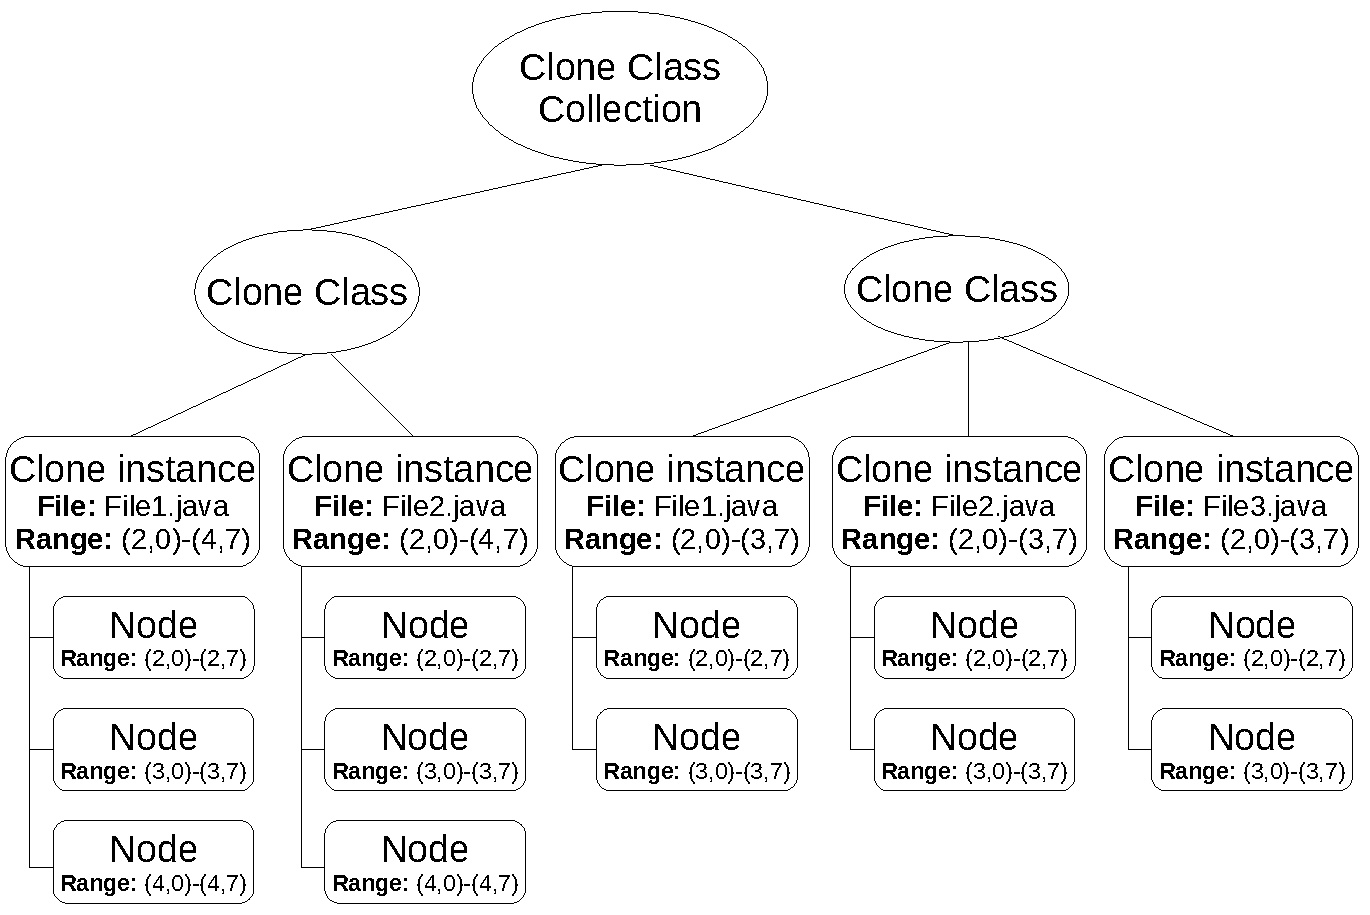
\includegraphics[width=1\columnwidth]{img/TerminologyExample}
  \caption{Tree representation of Figure~\ref{fig:cloneclasses} using the terminology of Table~\ref{tab:clone-terminology}}
  \label{fig:terminologyexample}
\end{figure}

\subsection{Clone Classes vs Clone Pairs}\label{sec:classesvspairs}
In Table~\ref{tab:clone-terminology} we introduced the concept of clone classes. Clone classes consist of any number of clone instances. Some clone detection tools detect ``clone pairs'' instead, which consider each pair of clone instances separately. There are different arguments in the literature whether clone pairs or clone classes should be considered for detection.

We decided to focus on \textit{clone classes} for our study, because of their advantages for refactoring. Clone pairs do not provide a general overview of all entities containing the clones, with all their related issues and characteristics~\cite{fontana2012duplicated}. Although clone classes are harder to manage, they provide all information needed to plan a suitable refactoring strategy, since this way all instances of a clone are considered. Another issue that results from grouping clones by pairs: the amount of clone references increases according to the binomial coefficient formula (two clones form a pair, three clones form three pairs, four clones form six pairs, and so on), which causes a heavy information redundancy~\cite{fontana2012duplicated}.

\section{Clone Types} \label{chap:backgroundclonetypes}
Duplication in code is found in many different forms. Most often duplicated code is the result of a programmer reusing previously written code \cite{haefliger2008code, baxter1998clone}. Sometimes this code is then adapted to fit the new context. To reason about these modifications, several clone types have been proposed. These clone types are described in Roy et al \cite{roy2007survey}:
\begin{displayquote}
\textbf{Type I:} Identical code fragments except for variations in whitespace (may be also variations in layout), and comments.\\
\textbf{Type II:} Structurally/syntactically identical fragments except for variations in identifiers, literals, types, layout, and comments.\\
\textbf{Type III:} Copied fragments with further modifications. Statements can be changed, added or removed in addition to variations in identifiers, literals, types, layout, and comments.
\end{displayquote}
A higher type of clone means that it is harder to detect and refactor. Many studies adopt these clone types, analyzing them further and writing detection techniques for them \cite{sajnani2016sourcerercc, kodhai2010detection, van2019novel}.

\section{Refactoring techniques}
In Martin Fowler's popular ``Refactoring'' book \cite{fowler2018refactoring}, he exclaims that \textit{``if you see the same code structure in more than one place, you can be sure that your program will be better if you find a way to unify them''}. He describes several techniques to deal with duplication, dependent on the context of the clone. In this section, we describe the techniques that we use in this study.

\subsection{Extract Method}
Current clone refactoring research shows that the ``Extract Method'' refactoring technique can refactor most duplication problems \cite{fontana2015duplicated, tsantalis2015assessing, white2016deep}. ``Extract Method'' moves matching functionality in method bodies to a common place, namely a new method \cite{fowler2018refactoring}. An example of this procedure is displayed in figure \ref{fig:extractmethod}.

\begin{figure}[H]
\begin{parcolumns}{2}
\colchunk[1]{
\begin{javacode}
// Original
public void doStuff(){
|\highlightYellow|  doA();
|\highlightYellow|  doB();
  doC();
|\highlightYellow|  doA();
|\highlightYellow|  doB();
}
\end{javacode}}
\colchunk[2]{
\begin{javacode}
// Refactored
public void doStuff(){
|\highlightYellow|  doAandB();
  doC();
|\highlightYellow|  doAandB();
}

public void doAandB(){
  doA();
  doB();
}
\end{javacode}}
\end{parcolumns}
\caption{Refactoring a clone class through method extraction.}
\label{fig:extractmethod}
\end{figure}

\subsection{Move method}
In the example of the previous section, both duplicated parts are in the same method. However, a study by Fontana et al. \cite{fontana2015duplicated} shows that this is most often not the case. Based on the relation between clone instances, the extracted method must be moved to be accessible by all locations of the clone instances. This can require different techniques.

\subsubsection{Pull up method}
A refactoring technique to move a method up in its inheritance structure is called ``Pull up method'' \cite{fowler2018refactoring}. This way, if cloned methods are related in any way through inheritance, they can be called by both classes by placing the method in a class they both have in common. This way it is possible to refactor both fully cloned methods (by just pulling up the method) and partially cloned methods (by first performing method extraction and then pulling up the refactored method). An example of this refactoring technique is shown in Figure~\ref{fig:pullupmethod}.

\begin{figure}[H]
\begin{parcolumns}{2}
\colchunk[1]{
\begin{javacode}
// Original
class Vehicle{
  void start(){
|\highlightYellow|    putKeyIn();
|\highlightYellow|    turnKey();
    drive();
  }
}

class Car extends Vehicle{
  void startEngine(){
|\highlightYellow|    putKeyIn();
|\highlightYellow|    turnKey();
  }
}
\end{javacode}}
\colchunk[2]{
\begin{javacode}
// Refactored
class Vehicle{
  void start(){
|\highlightYellow|    startEngine();
    drive();
  }

  void startEngine(){
|\highlightYellow|    putKeyIn();
|\highlightYellow|    turnKey();
  }
}

class Car extends Vehicle{
}
\end{javacode}}
\end{parcolumns}
\caption{Refactoring a clone class using ``Pull Up Method''.}
\label{fig:pullupmethod}
\end{figure}

\subsubsection{Create class abstraction based on implicit relations}
Duplication in source code is an implicit relation between fragments of source code. If two classes have many of these implicit relations, then the implementation should be refactored to make this relation explicit \cite{fowler2018refactoring}. If the classes do not yet have a parent/superclass, a parent class can be created and the common functionality can be placed in this newly created class. This makes the relationship between these classes explicit and reduces duplication.

\begin{figure}[H]
\begin{parcolumns}{2}
\colchunk[1]{
\begin{javacode}
// Original
class Truck{
  void startEngine(){
|\highlightYellow|    putKeyIn();
|\highlightYellow|    turnKey();
  }
}

class Car{
  void startEngine(){
|\highlightYellow|    putKeyIn();
|\highlightYellow|    turnKey();
  }
}
\end{javacode}}
\colchunk[2]{
\begin{javacode}
// Refactored
class Vehicle{
  void startEngine(){
|\highlightYellow|    putKeyIn();
|\highlightYellow|    turnKey();
  }
}

class Truck extends Vehicle{
}

class Car extends Vehicle{
}
\end{javacode}}
\end{parcolumns}
\caption{Refactoring a clone class using ``Create class abstraction''.}
\label{fig:createclassabstraction}
\end{figure}

\subsubsection{Providing default implementations for common functionality}
In Java, C\#, Python, and possibly other object-oriented languages, the programmer can create interfaces of which a class can implement any number. Such interfaces can (in Java, C\#, and Python) provide default implementations for common functionality \cite{mohnen2002interfaces}. This allows making the relation between classes explicit and reduce duplication. It can be used in instances where creating a new parent class for duplicated classes is undesirable. An example of this is shown in Figure~\ref{fig:createinterfaceabstraction}, in which two unrelated types (Human and Radio) share a common property (making a sound).

\begin{figure}[H]
\begin{parcolumns}{2}
\colchunk[1]{
\begin{javacode}
// Original
class Human implements MakesSound{
  void broadcastNews(){
|\highlightYellow|    sayNews();
|\highlightYellow|    sayWeather();
  }
}

class Radio implements MakesSound{
  void broadcastNews(){
|\highlightYellow|    sayNews();
|\highlightYellow|    sayWeather();
  }
}

interface MakesSound{
  void sayNews();
  void sayWeather();
}
\end{javacode}}
\colchunk[2]{
\begin{javacode}
// Refactored
class Human implements MakesSound{
}

class Radio implements MakesSound{
}

interface MakesSound{
  default void broadcastNews(){
|\highlightYellow|    sayNews();
|\highlightYellow|    sayWeather();
  }

  void sayNews();
  void sayWeather();
}
\end{javacode}}
\end{parcolumns}
\caption{Refactoring a clone class creating a default implementation for common functionality.}
\label{fig:createinterfaceabstraction}
\end{figure}

\section{Internal and external classes}
In this study we differentiate between \textit{internal} and \textit{external} classes. Classes are the components of a software system that contain its functionality. When analyzing a software system, \textit{Internal classes} are classes that belong to this software system specifically, and its source code is included in the project.

\textit{External classes} are classes that a software system uses but do not belong to this specific software system (but to an external dependency). Most often these external dependencies are referenced in a file that its build automation system uses to fetch a projects' dependencies.

Regarding refactoring, a software system can often not change the source code of its dependencies. This can be a burden when an external dependency does not use proper abstractions that are required by a software system. In this study we consider external classes when choosing a refactoring technique, to be sure not to modify them.

\subsection{Maven}
For this study we perform an analysis of external dependencies, to derive more context for internally used concepts. As these external dependencies are most often not included in a software systems' source code, we must first use the projects' build automation system to gather the dependencies. To limit the scope of this process, we decided to focus on only the \textit{Maven}\footnote{Apache Maven is a build automation system mainly used for Java: \url{https://maven.apache.org/}} build automation system.

Maven is a build automation tool, mainly used with the Java programming language. Maven has a simple ecosystem to configure and fetch the binaries and source code of all software projects a given codebase is dependent on. Maven can also be used to run tests for the systems and to package the project as an executable file.

\section{(Object-Oriented) Programming Languages}
This section explains concepts, terminology, and jargon of (object-oriented) programming languages that we use in this study.

\subsection{AST} \label{sec:astbackground}
An Abstract Syntax Tree (AST) is a tree consisting of a hierarchical representation of the source code of a program. Detecting code clones on the AST of a program allows for a deeper understanding of the concepts that are being analyzed. Having an AST, we know how concepts in the code are related. This helps to determine in what classes and methods cloned code is found.

Having access to a programs' AST also helps in the process of refactoring. Moving AST nodes rather than textual modifications reduces error margins because the tree structure stays intact.

The AST consists of nodes of the following types (examples are for Java):
\begin{itemize}
  \item \textbf{Declarations}: Method-declaration, class-declaration, etc.
  \item \textbf{Statements}: If-statement, switch-statement, expression-statement, etc.
  \item \textbf{Expressions}: Variables, literals, method calls, variable assignments, etc.
  \item \textbf{Types}: Primitives, reference types, void, etc.
  \item \textbf{Clauses}: Catch-clause, else-clause, etc.
\end{itemize}

\subsection{Inheritance}
Object-Oriented programming languages use inheritance to model real-world relations between data concepts. Inheritance allows an object to inherit all functionality from another object. For instance, a ``Car'' object would inherit functionality and data from generalized concepts, such as ``Vehicle''. Using inheritance it is possible to reduce duplication, as multiple objects can inherit common functionality.

When looking at the inheritance structure of a program, we can get a deeper understanding of a programs' architecture. The use of inheritance to group common functionality and data is called ``Abstraction''. Duplication in source code can be a result of inadequate use of abstraction. Because of that, refactoring code clones might require to create such abstractions of common functionality.

\subsection{Code Quality}
Different programming languages have different ways to measure code quality. For object-oriented programming languages, this largely comes in the form of code smells (patterns that should be avoided) and design patterns (patterns which may improve code design and comprehensibility when used correctly).

\subsubsection{Code Smells}
Code smells are patterns in code that should be avoided because they harm system design. Duplicate code is, among many others, one example of a code smell. Having many code smells present in source code can significantly increase the maintenance costs of the source code or even render a software system unmaintainable. This increases technical debt: a debt present in the system the will have to be repaid at a later point of time. Such technical debt often comes at the expense of developing new features, fixing bugs and other aspects surrounding the functional behavior of a program.

\subsubsection{Design Patterns}
Most code smells have design patterns that can be used to mitigate the smell. For instance, duplicate code can be mitigated by using appropriate abstractions or refactoring duplicate code to a common place. Design patterns differ from refactoring methods in the sense that they are more about an architectural pattern rather than a certain kind of code modification.

\subsubsection{Maintainability Metrics}
Maintainability metrics are features of source code by which an indication of the maintainability of the source code can be measured. Heitlager at al. \cite{heitlager2007practical} propose a maintainability model that categorize the results of metrics into different ``score'' categories. For instance, with duplication, if 0-3\% of the project is duplicated, the project will get the highest score on a scale of 1 to 5 (only integers, no floating-point numbers). Such a maintainability model is intuitive for measuring the quality of a software system, especially large software systems with a lot of source code to base the metrics on. However, this maintainability model \cite{heitlager2007practical} lacks in measuring fine-grained changes: most small changes will not fall into a different category. Because of that, this model is less suitable for measuring the impact of single refactorings.

\subsection{Java}
We run all our experiments on projects written in Java. Because of that, we get some information that is specific to Java systems. Additionally, we perform automated refactorings on Java systems, which requires the use of Java language concepts. These are explained in this section. Many of these concepts also exist in other programming languages, but often not in all.

\subsubsection{Interfaces}
Java uses the concept of interfaces to loosely couple a specification and its implementation. Interfaces are specifications about what a (group of) objects do. Often, methods don't need an entire object, but just use a few properties of it. Because of that, Java recommends programming to an interface rather than an implementation. This means that we should use abstractions of expected functionality rather than complete implementations of functionality. This can make switching implementations at a later point in time easier.

Often, duplication is the result of inappropriate use of abstractions. Two methods might describe operations on types following the same contract, but because of a lack of abstraction, the programmer may choose to clone such methods. This will result in duplicated methods with minor modifications to match a different implementation. Such duplicates can be mitigated by using proper abstractions, of which one option is to program methods against interfaces (contracts of expected functionality) rather than their full implementations.

\subsubsection{Packages}
Packages (sometimes called ``modules'' in other programming languages) are hierarchical groupings of related concepts. For instance, all UI logic in an application might go into the ``ui'' package. The ``ui'' package can have a subpackage named ``keyhandling'' for all keyboard input related operations. These packages contain package-level declarations, like classes and interfaces. Names of class-level declarations must be unique within the package. %However, duplicate declaration names may exist in subpackages and parent packages.

In Java, all declarations used from outside the package a declaration is in, must be \textit{imported}. Importing a declaration from outside the current package goes by the fully qualified identifier (FQI) of the declaration. The FQI of a declaration gives a unique identifier for a symbol in a codebase. For instance, if our ``keyhandling'' package would contain a ``KeyHandler'' class, its fully qualified identifier would be ``ui.keyhandling.KeyHandler''.

\subsubsection{Visibility}
In Java, we can protect declarations from being used in scopes in which they are supposed to be used. If a method should only be used within the class itself, we can give it a ``private'' visibility. If a method is to be used by its children in its inheritance hierarchy, we can set its visibility to ``protected''. If a method is supposed to be part of the public contract of an object, we can set it to ``public'' visibility. Alternatively, there is ``package'' visibility, for declarations that should only be referenced within the same package. This allows control over what parts of an application should be able to access what declarations.
